%% \documentclass{report}
%% \usepackage{fullpage}
%% \usepackage{tikz}
%% \usepackage[utf8]{inputenc}
%% \usepackage[OT1]{fontenc}

%% \begin{document}

%% \scalebox{0.6}{

\begin{tikzpicture}

\draw[white] (21,3.5) rectangle (26,-3);


\only<5->{
%global
\draw[fill=white] (21,3.5) rectangle (26,-3);
\draw[fill=white] (18,3) rectangle (23,-3.5);
\draw[fill=white] (15,2.5) rectangle (20,-4);
\draw[fill=white] (12,2) rectangle (17,-4.5);
\draw[fill=white] (9,1.5) rectangle (14,-5);
\draw[fill=white] (6,1) rectangle (11,-5.5);
\draw[fill=white] (3,0.5) rectangle (8,-6);
}

%local
\draw[fill=white] (0,0) rectangle (5,-6.5);

\only<2-4>{
%row
\draw[fill=blue!20] (0.5,-1.5) rectangle (4.5,-2.5);
}

\only<3-4>{
%copy
\draw[fill=blue!20] (0.5,-5) rectangle (4.5,-6);
}
\only<3>{
\draw[->,very thick] (4.6,-2) to[out=360,in=360] (4.6,-5.5);
}

\only<4>{
%column
\draw[fill=black!10] (2.5,-0.5) rectangle (3.5,-4.5);
\draw[fill=red!50] (2.5,-5) rectangle (3.5,-6);
}

\only<1-4>{
\draw (0.5,-0.5) rectangle (4.5,-4.5);
\draw (0.5,-5) rectangle (4.5,-6);
\draw (0.5,-1.5) -- (4.5,-1.5);
\draw (0.5,-2.5) -- (4.5,-2.5);
\draw (0.5,-3.5) -- (4.5,-3.5);
\draw (1.5,-0.5) -- (1.5,-4.5);
\draw (2.5,-0.5) -- (2.5,-4.5);
\draw (3.5,-0.5) -- (3.5,-4.5);
\draw (1.5,-5) -- (1.5,-6);
\draw (2.5,-5) -- (2.5,-6);
\draw (3.5,-5) -- (3.5,-6);
}

\only<6->{
%global
\draw[fill=red!50] (2.5,-1.5) rectangle (3.5,-2.5);
\draw[fill=red!50] (5.5,-1) rectangle (6.5,-2);
\draw[fill=red!50] (8.5,-0.5) rectangle (9.5,-1.5);
\draw[fill=red!50] (11.5,0) rectangle (12.5,-1);
\draw[fill=red!50] (14.5,0.5) rectangle (15.5,-0.5);
\draw[fill=red!50] (17.5,1) rectangle (18.5,0);
\draw[fill=red!50] (20.5,1.5) rectangle (21.5,0.5);
\draw[fill=red!50] (23.5,2) rectangle (24.5,1);
}

\only<7>{
\draw (2,-8) rectangle (26,-9);
\draw (5,-8) -- (5,-9);
\draw (8,-8) -- (8,-9);
\draw (11,-8) -- (11,-9);
\draw (14,-8) -- (14,-9);
\draw (17,-8) -- (17,-9);
\draw (20,-8) -- (20,-9);
\draw (23,-8) -- (23,-9);

\draw[->,very thick] (3,-2.6) -- (3,-8.4);
\draw[->,very thick] (6,-2.1) -- (6,-8.4);
\draw[->,very thick] (9,-1.6) -- (9,-8.4);
\draw[->,very thick] (12,-1.1) -- (12,-8.4);
\draw[->,very thick] (15,-0.6) -- (15,-8.4);
\draw[->,very thick] (18,-0.1) -- (18,-8.4);
\draw[->,very thick] (21,0.4) -- (21,-8.4);
\draw[->,very thick] (24,0.9) -- (24,-8.4);
}

%% \foreach \i in {0,...,15} {
%%   \foreach \j in {-20,...,0} {
%%     \node[red] at (\i,\j) {\i,\j};
%%   }
%% }


\end{tikzpicture}

%% }

%% \end{document}
